\RequirePackage{luatex85}
\documentclass{standalone}

\usepackage{fontspec, unicode-math}
\setsansfont[Scale=MatchLowercase]{TeX Gyre Heros}
\setmathfont{TeX Gyre Termes Math}

\usepackage{tikz}
\usetikzlibrary{arrows.meta}
\usetikzlibrary{calc}
\usetikzlibrary{positioning}

\tikzset{
  every picture/.style={font={\sffamily\normalsize}, >=stealth},
  every pin edge/.style={black}}

\begin{document}

  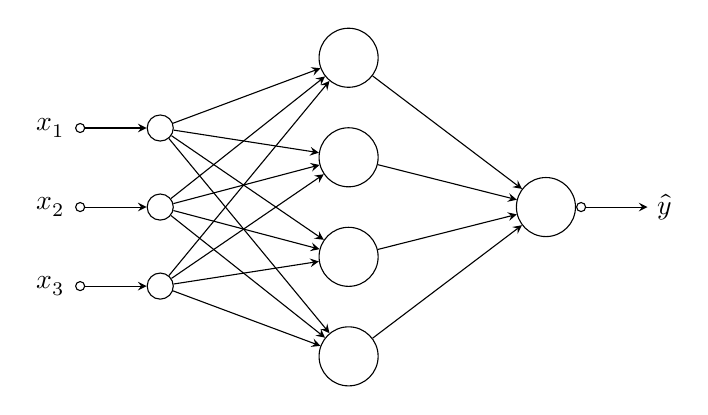
\begin{tikzpicture}[pin distance=6ex, node distance=0.5cm and 2cm,
    input/.style={draw, circle},
    unit/.style={draw, circle, minimum size=0.75cm}]

    \begin{scope}
      \node[unit] (HA) {};
      \node[unit] (HB) [below=of HA] {};
      \node[unit] (HC) [below=of HB] {};
      \node[unit] (HD) [below=of HC] {};
    \end{scope}

    \begin{scope}[pin edge={<-{Circle[open]}}]
      \node[input] (IA) [pin=left:$x_{1}$, below left=of HA] {};
      \node[input] (IC) [pin=left:$x_{3}$, above left=of HD] {};
      \node[input] (IB) at ($(IA)!0.5!(IC)$) [pin=left:$x_{2}$] {};
    \end{scope}

    \begin{scope}[pin edge={{Circle[open]}->}]
      \node (O1) [right=of HA] {};
      \node (O2) [right=of HD] {};
      \node[unit] (OA) at ($(O1)!0.5!(O2)$) [pin=right:$\hat{y}$] {};
    \end{scope}

    \path[->] (IA) edge (HA) edge (HB) edge (HC) edge (HD);
    \path[->] (IB) edge (HA) edge (HB) edge (HC) edge (HD);
    \path[->] (IC) edge (HA) edge (HB) edge (HC) edge (HD);

    \path[->] (HA) edge (OA);
    \path[->] (HB) edge (OA);
    \path[->] (HC) edge (OA);
    \path[->] (HD) edge (OA);
  \end{tikzpicture}

\end{document}
